% !TeX root = ../main.tex
% Add the above to each chapter to make compiling the PDF easier in some editors.

\chapter{Approach}\label{chapter:Approach}


\section{System Design }
A system design can be broadly described as an architecture of the system, which includes an explanation of each hardware component of the system, the connection between these components if there is any, and the data flowing between these components. Moreover, it gives an idea of the whole system but not its exact functionality, hence, giving a simple understanding of the architecture without jumping into much detail.\\


\subsection{Components}
\label{sub:components}
Below, each component of the proposed system design is explained.

\subsubsection{Node}
\label{subsub:node}
%The first set of components to explain are the sensors, they refer to objects that detect certain change in the environment and converts these changes into digital data and 
%which refer to objects that can detect certain changes in the environment and converts them to digital data, 
A Node is one of the core components of this design, it is a small computer device of low storage and computation capacity compared to nowadays portable computers, commonly a \textit{Raspberry Pi} but could be any other device. It is connected to several sensors which typically detect certain changes in the environment and converts it into digital data, for instance, Gas sensor, Temperature sensor or a Camera. Then, the device either stores the data into a local database, performs a computation locally, does both or even asks other nodes to do computation instead, however, an assumption about which sensors or specifications does a specific node  possess can not be made, meaning, each node might not have the exact number or types of sensors because each node may be deployed in a different timing or context. Thus, each node has a configuration file specifying its capabilities. A typical node is shown in figure \ref{fig:node}

\begin{figure}[H]
	\centering
	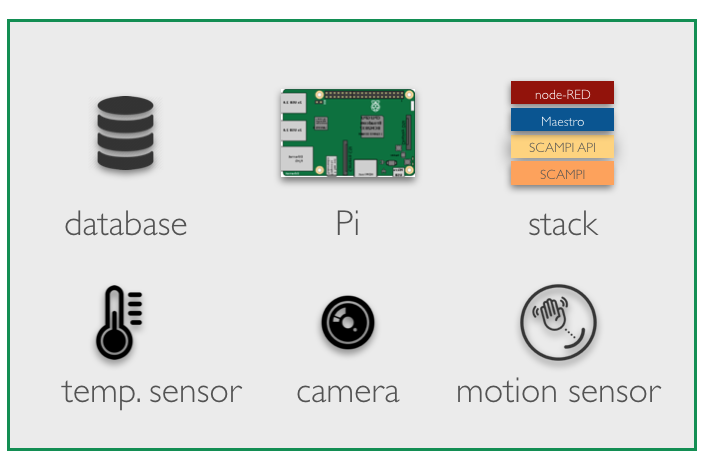
\includegraphics[scale=0.4]{images/node.png}
	\caption{A typical node in the system}
	\label{fig:node}
\end{figure}

\subsubsection{High Performance  Units }

CPUs in the proposed system nodes in \ref{subsub:node}. An example of a high processing unit is  a Graphics Processing unit \textit{GPU}.

\begin{figure}[H]
	\centering
	
\includegraphics[scale=0.7]{images/gpu.png}
	\caption{Figure denoting a Graphics Processing Unit GPU}
	\label{fig:gpu}
\end{figure}

\subsubsection{Network}
\label{subsub:network}
A Network in this design is a set of connected components which are capable of communicating and therefore allowing data sharing between them.
\begin{figure}[H]
	\centering
	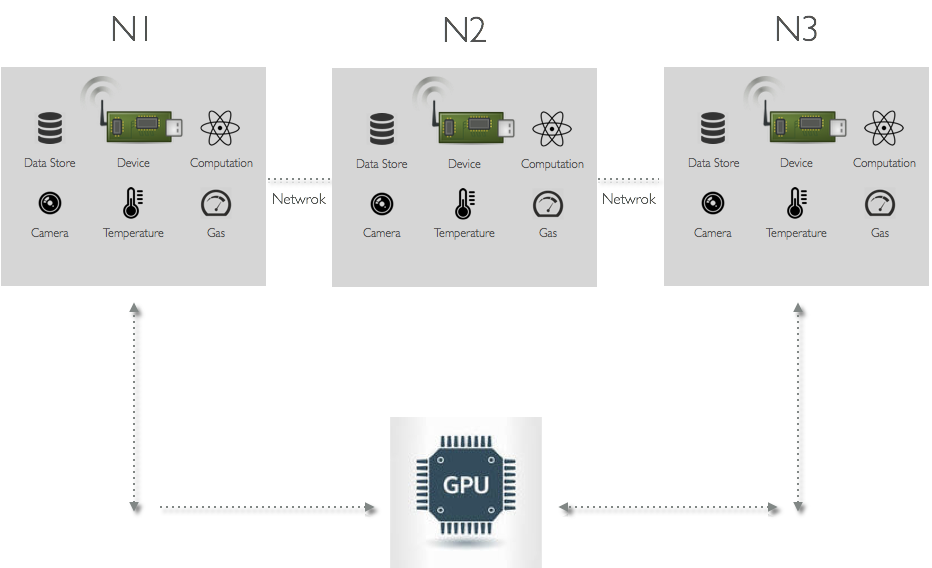
\includegraphics[scale=0.4]{images/network.png}
	\caption{A network consisting of three connected nodes and a GPU}
	\label{fig:network}
\end{figure}
-- TODO: 
Emphasis the difference between persistent and non persistent network links in system design.

\subsubsection{Mobile Device}
A Mobile Device in this context is any device that can connect to the network containing the nodes and is allowed to  carry data from one network to another, hence, allowing a form of data sharing between networks or nodes which are not connected.

\begin{figure}[H]
	\centering
	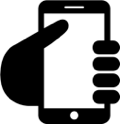
\includegraphics[scale=0.3]{images/mobile.png}
	\caption{Figure denoting a Mobile Device}
	\label{fig:mobile}
\end{figure}



\subsection{Connectivity and Data Flow}
A Network described in \ref{subsub:network}, is a simple form of connectivity between components, however, components and specifically nodes are not necessarily connected, sometimes they are just a standalone component that cannot share any information via direct connectivity, also, networks could be disconnected as well, meaning, a network might not be connected to the whole system, thus, is a standalone network. In these cases, a mobile device could help in carrying information and data between these disconnected nodes or networks. 

\begin{figure}[H]
	\centering
	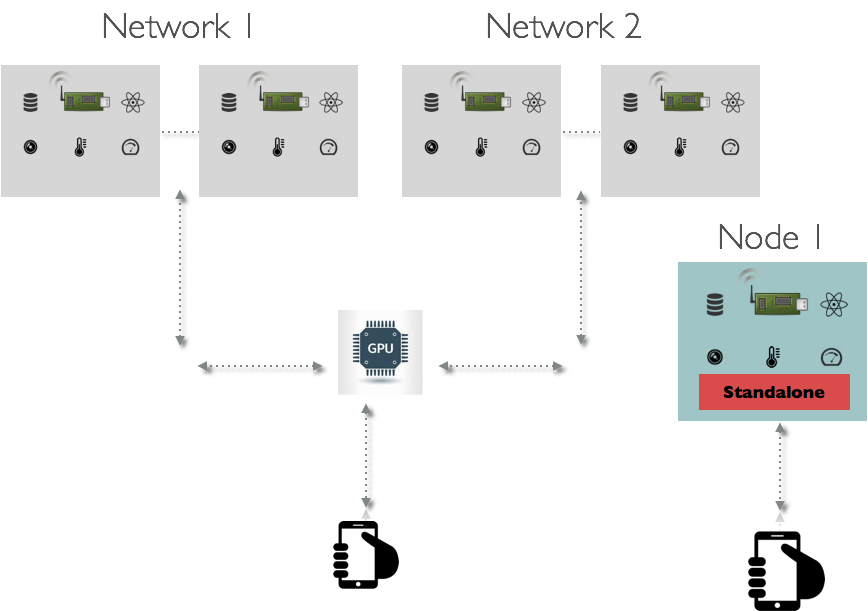
\includegraphics[scale=0.5]{images/system.png}
	\label{fig:system}
	\caption{Two networks connected with a GPU and one standalone network}
\end{figure}





\section{Use Cases}
\section{Requirements}
The framework should
\begin{itemize}
	\item  send computations to all or selected nodes.
	\item  allow computations to carry custom dependencies.
	\item  allow communication between nodes in a publish-subscribe manner.
	
	\item  carry computations forward even without an end-to-end path between sender and receiver.
	\item  allow computations to receive data as an input or publish data as an output using the communication layer.
	
	\item  send a computations to nodes according to their computation capabilities, available sensors and actuators.
	
	\item  send computations to  specific nodes with a given global identifiers.
	
	\item  allow computations to be composable locally and globally.
	
\end{itemize}

The computations should
\begin{itemize}
	\item  be able to access their dependencies.
	\item  be triggered either by a scheduler or at-will.
	\item  persist data in any form.
	\item  access hardware resources such as camera, sensors and actuators.
	\item  be pervasive and act on their own.
\end{itemize}
%It is believed that development of smart pervasive computing devices that uses sensors and actuators are mainly grouped into smaller disconnected architectures and thus hard to create a composite framework in which all devices can communicate and integrate\cite{5470524}. In order to tackle this problem and to ensure that our computational model design is dynamic and flexible enough, we must ensure that our model is composable. By Composability we mean that computational models should be able to communicate, send and receive input and output data. 




\section{Summary}



